\documentclass[11pt,a4paper]{article}
\usepackage[text={6.5in,10in},centering,a4paper]{geometry}
\usepackage{amssymb,amsmath} % Equations
\usepackage{tabularx} % Tables
\usepackage{graphicx,color} % Graphics, Figures
\usepackage[tight,footnotesize]{subfigure}
\usepackage{pgfgantt} % for gantt chart
\usepackage{indentfirst}
\usepackage{hyperref}
\usepackage{amsmath} % for large blaces
\usepackage{esvect} % easy vector
\usepackage{etoolbox} % for bibliography
\usepackage{pdflscape} %landscape
\patchcmd{\thebibliography}{\section*}{\section}{}{}

\graphicspath{{figures/}} % create a director 'figures' in your local dir and all pics are kept here

\title{
  \textbf{Senior Project Proposal 2102490 Year 2017}  \\[2ex]
  Analysis and Design of Planar Phased Array Antenna for \\[1ex]
  5 GHz Applications
}
\author{\textbf{Norawit Nangsue ID 5730289021} \\[1ex]
\textbf{Advisor: Assist. Prof. Tuptim Angkaew} \\[1ex]
\textbf{Department of Electrical Engineering, Faculty of Engineering} \\[1ex]
\textbf{Chulalongkorn University}
}
\date{\today}

\renewcommand\familydefault{\sfdefault} % set to San Serif series

\begin{document}
  \maketitle
  \tableofcontents
  \newpage
  \section{Introduction}
    %Requirement
    \indent The advances of technologies now ahead through now wouldn't be happened without a communication systems.
            In such today, wireless communication is covering almost everywhere in the world. One of the most important
            thing in the communication system is the antenna. Because it could be able to radiate or receive power into the air.
            With these abilities, we may use it to send or receive those infomation that we want to. As we know, just a wire
            could be used as an antenna technically. However, its property may not be good for every requirement or application.

    %Frequency        
    \indent The freedom of using frequency bands bring us to the world of technologies. Back to 1947, in the International Telecommunications
            Conference of the ITU in Atlantic City established the first lot of ISM(Industrial, Scientific and Medical) bands which allows us
            to use those frequency without asking for a permission. For example, the microwave oven, we never have to ask for any government's 
            allowance to use the microwave which radiates the electromagnetic wave at the frequency of 2.45 GHz to our food because this 
            frequency is in ISM bands.

    %Directivity
    \indent There are many methods to increase the range of the antenna. The easiest one is increasing more power. However, if we just want
            to send a message from a station to another station, there will be a huge power loss on the air at the direction that we don't
            really need to send to. In a good practical, engineers design antennas that their property is focusing on only one direction which
            is called Directivity. Therefore, a high directivity antenna can be able to send more distance than the ordinary one.

    %Phased Array Antenna
    \indent Considering a droplet drops on the surface of the water, there will be a circular wave spreading out from the origin.
            If there are multiple droplets in a row, those wave will be constructed and destructed depends on location and it'll
            reform like a seacoast wave. So this will make a more powerful wave from 2 sources. Moreover, the direction can also
            be changed by controling how droplets fall onto the surface. The same as the array of antennas, if we can control each
            element's phase so we will be able to control antenna's directivity upon our desire. 

    %Easy to use & Size
    \indent If we want to make a device that everyone agrees on carrying to everywhere, basically, it must be small, thin and cheap.
            To response to this demand, there is a flat composite material which composed of woven fiberglass cloth available in the market.
            It's FR4(a grade designation assigned to glass-reinforced epoxy laminate sheets, tubes, rods and printed circuit boards).
            Engineers usually uses FR4 as a microstrip. It could be any type of microwave circuits including antennas.
    
    %Summary
    \indent Therefore, there are a lot of basic constraints up depends on which application we use. As from the title of this proposal,
            Analysis and Design of Planar Phased Array Antenna for 5 GHz Applications, this project consists reviewing the
            past literature, derived formula, empirical formula and try to using all of these knowledges to design the array of antenna with
            phase-controlled at the ISM band(5.8 GHz)
  
  \newpage

  \section{Objectives}
    \indent The main objective of this project is to study about the analysis of the phased array antenna, and check whether the result is the
            same. It consists of several tasks combining together.
    \begin{itemize}
      \item Review past lituratures
      \item Compare techniques
      \item Design the antennas and circuits
      \item Simulate the antennas
      \item Test and find its result
      \item Compare the antenna results with the analysis method
    \end{itemize}
    \indent for the full procedure flowchart it'll be shown in the methodology section.
   
  \newpage
  
  \section{Methodology}
    \indent This is the project procedure flowchart
    \begin{figure}[ht]
      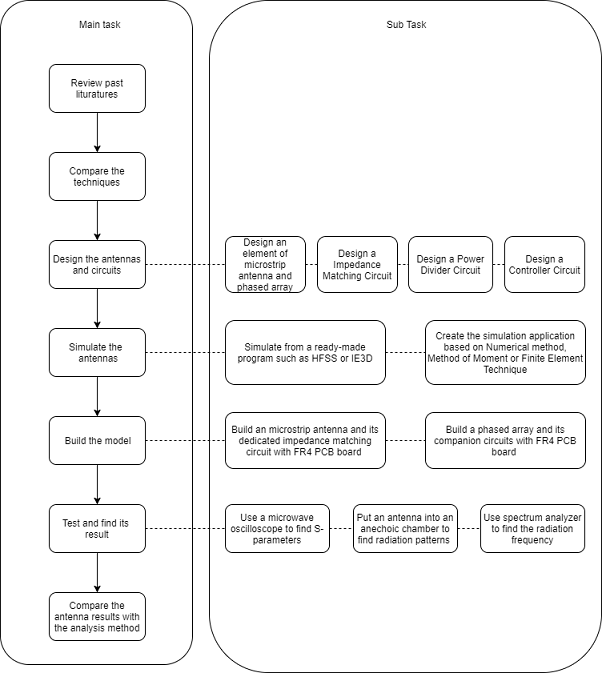
\includegraphics{flowchart_ml.png}
        \centering
        \caption{The project procedure flowchart is shown above.}
    \end{figure}
    
    \newpage
    %\indent This section will provide a full analysis of designing a microstrip antenna and a phased array antenna.
    
    \subsection{Basic Dimension Design of The Microstrip Antenna}
      \indent a dimension of microstrip antenna can be designed easily with this expressions\cite{NoK:05}.
      \begin{equation}
        L = \frac{c}{2f_0\sqrt{\epsilon_r\mu_r}} - 2\Delta l 
        W = \frac{c}{2f_0}
      \end{equation}
      \indent where $L$ and $W$ are the dimensions of an antenna\\[1ex]
      \indent $f_0$ is the resonance frequency\\[1ex]
      \indent $\epsilon_r$ is the relative dielectric constant\\[1ex]
      \indent $\mu_r$ is the relative magnetic constant\\[1ex]
      \indent $c$ is the speed of light in free space\\[1ex]
      \indent $\Delta l$ is the fringing effect at the edge of the antenna\\[3ex]
      \indent However from \cite{CoB:05} the best width should be
      \begin{equation}
        W = \frac {1} {2 f_r \sqrt{\mu_{0} \epsilon_{0}}}\sqrt{\frac{2}{\epsilon_{r} + 1}} = \frac{\upsilon_{0}}{2f_{r}}\sqrt{\frac{2}{\epsilon_{r} + 1}}
      \end{equation}
      \indent where $\upsilon_{0}$ is the free-space velocity of light
    
  \newpage

    \subsection{Transmission Line Model}
      \indent Transmission Line Model is considered as the easiest way to analyze the description of the
              rectangular microstrip patch.
      \begin{figure}[ht]
        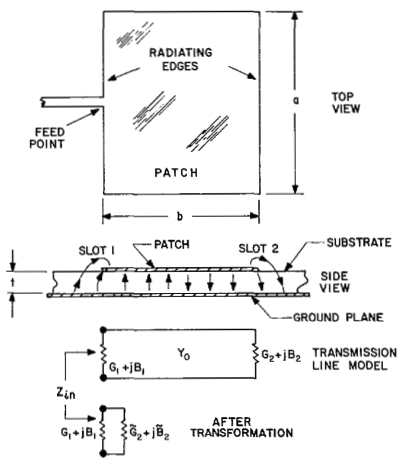
\includegraphics{tmmodel.png}
          \centering
          \caption{The antenna at top view, side view, and its transmission line model\cite{CaM:81}}
          %\label{fig:10}
      \end{figure}

      \subsubsection{Slot admittance}
        \indent The slot admittance is given by \cite{CaM:81}
        \begin{equation}
          G_1 + jB_1 \cong \frac{\pi {a}}{\lambda_0 z_0}[1 + j(1-0.636\ln{k_0w})]
        \end{equation}
        \indent where $a$ is the length of the patch antenna, $\lambda_0$ is free space wavelength,
                $k_0 = frac{2\pi}{\lambda_0}$, and $w$ is the slot width which is approximately
                equals to the thickness of the substrate $t$ 

      \subsubsection{Characteristic admittance}
        \indent Assume that there is no field variation along the edge of plate, so the characteristic admittance is given by \cite{CaM:81}
        \begin{equation}
          Y_0 = \frac{a\sqrt{\epsilon_r}}{tz_0}
        \end{equation}
        \indent where $t$ is the substrate thickness and the impedance of free space which is $\sqrt{\frac{\mu_0}{\epsilon_0}}$

      \subsubsection{Total Admittance \& Resistance at Resonance frequency}
        \indent By using Smith chart to get the length that will reflute out the imaginary part. Then, the total impedance would be
        \begin{equation}
          Y_{in} = 2G_1
        \end{equation}
        \indent Typically, $b$ should be at $0.48\lambda_d$ to $0.49\lambda_d$ because of the imaginary part reflution
                and the compensation of the fringing effect that cause an extra effective length. Also, $a$ should be around
                $0.5\lambda_0$ as well to get the best power radiation.  \\[1ex]
        \indent After complete the calculation of the admittance from the above parameters, so that the admittance
                $G_1 = 0.00417$ mhos. Then the input impedance of the antenna would be
        \begin{equation}
          Z_{in} = \frac{1}{2G_1} = 120 \indent \Omega
        \end{equation}

      \subsubsection{Resonance frequency}
        \indent The resonant frequency is found from
        \begin{equation}
          f_r = \frac{c}{\lambda_d\sqrt{\epsilon_r}} = q\frac{c}{2b\sqrt{\epsilon_r}}
        \end{equation}
        \indent where $q$ is the accurary of the resonant frequency and could easily determined by measuring $f_r$ \cite{CaM:81}
      
        \subsubsection{Summary}
        \indent The transmission line model is very easy to design and calculate parameters. However, the transmission line
                model is hardly to adapt with the other shape of the patch or. Also, this model is lack of accurate data.
                In order to find more precise infomation about the antenna, the Cavity model will be introduced 
                in the next section which is much more accurate than this one.\cite{CaM:81,NoK:05}
  \newpage

    \subsection{Cavity Line Model}
    \indent The cavity model has more accurate formulation for the input impedance, resonance with a little
            increase of mathematical complexity.\cite{CaM:81}
    \begin{figure}[ht]
      \label{cavitymodel}
      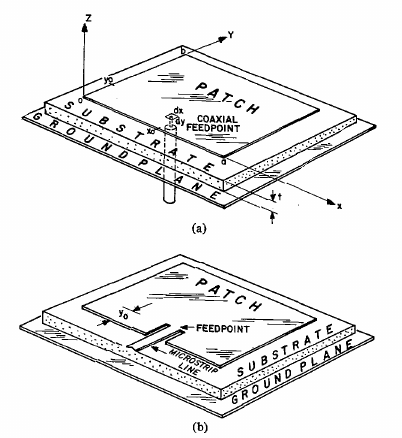
\includegraphics{cavitymodel.png}
      \centering
      \caption{(a) Microstrip patch with inset coaxial feed
               (b) Microstrip patch with inset transmission-line feed
              }
    \end{figure}

      \subsubsection{General form of electric field}
        \indent Considering a rectangular patch with width $a$ and length $b$ over a ground plane with $t$ substrate
                thickness and a dielectric constant $\epsilon_r$. With the relatively short thickness of the substrate,
                the electric field will be in z-direction with $TM_{mn}$ interior modes so that\cite{CaM:81}
        \begin{equation}
          \label{GeneralE}
          E_z = \sum_m\sum_n A_{mn}e_{mn}(x,y)
        \end{equation}
        \indent where $A_{mn}$ are the mode amplitude coefficients and $e_{mn}$ are z direction electric mode vectors.
        \indent However, the mode that is used in the antenna is just only $TM_{10}$ so the equation can easily write as
        \begin{equation}
           E_z = A_{10}e_{10}(x,y)
        \end{equation}

      \subsubsection{Nonradiating cavity with perfect open-circuit wall equation of electric field}
        \indent With a calculation from boundary condition, it could be found that
          \begin{equation}
            \label{OpenE}
            e_{mn}(x,y) = \frac{\chi_{mn}}{\sqrt{\epsilon abt}}\cos{k_nx}\cos{k_my}
          \end{equation}
        \indent with
          \begin{equation}
            \chi_{mn}=
            \begin{cases}
              1       , & m = 0\quad     \text{and}\quad  n = 0 \\
              \sqrt{2}, & m = 0\quad     \text{ or }\quad  n = 0 \\
              2       , & m \neq 0\quad  \text{and}\quad  n \neq 0
            \end{cases}
          \end{equation}

      \subsubsection{Wavenumber}
        \indent The homogenous wave function and the eigenvalues must be complied with the seperation equation
        \begin{equation}
          \label{kmn}
          k_{mn}^2 = \omega_{mn}^2\mu\epsilon = k_n^2 + k_m^2\\
        \end{equation}
        \indent in the case of nonradiating cavity
        \begin{equation}
          k_{n} = \frac{n\pi}{a}\\
          k_{m} = \frac{m\pi}{b}
        \end{equation}

      \subsubsection{Nonradiating cavity with perfect open-circuit wall equation of magnetic field}
        \indent From Maxwell-Faraday equation
        \begin{equation}
          \nabla \times \vv{E} = - \frac {\partial{\vv B}} {\partial t}
        \end{equation}
        \indent or in phasor form,
        \begin{equation}
          \nabla \times \vv{E} = -j\omega{\vv B}
        \end{equation}
        \indent after substitute the electric field equation, the magnetic field will be
        \begin{equation}
           \vv{h}_{mn} = \frac{1}{j\omega\mu}\frac{\chi_{mn}}{\sqrt{\epsilon abt}}(\vv{x}k_m\cos{k_nx}\sin{k_my} - \vv{y}k_n\sin{k_n}{x}\cos{k_m}{y})
        \end{equation}
        \indent For nonradiating case, the boundary condition $\vv{n} \times \vv{h}_{mn} = 0$ is satisfied on every walls.
                But, in radiating case, $\vv{h}_{mn}$ will not have a zero tangential on the cavity sidewall anymore.
                However, those pertubation from radiating effect cause just a little error on $e_{mn}$\cite{CaM:81}
      
      \subsubsection{Mode Coefficient}
        \indent From z-direction current, with the current probe $I_{0}$ at the location $(x_0,y_0)$ as in the
                figures illustrates in \ref{cavitymodel}. The coefficients from each mode can be obtained from
        \begin{equation}
          A_{mn} = \frac{j\sqrt{\mu\epsilon}k}{k^2-k_{mn}^2} \int\int\int\vv{J} \cdot \vv{e}_{mn} dv
        \end{equation}
        \begin{equation}
          \label{ModeCoeff}
          A_{mn} = jI_0 \sqrt{\frac{\mu t}{ab}} \frac{k\chi_{mn}}{k^2-k_{mn}^2} G_{mn} \cos{k_my_0}\cos{k_nx_0}
        \end{equation}
        \indent where
        \begin{equation}
          G_{mn} = \frac{\sin(n\pi d_x/2a)}{n\pi d_x/2a}\frac{\sin(m\pi d_y/2b)}{m\pi d_y/2b}
        \end{equation}
        \indent and
        \begin{equation}
          k_{mn} = \widetilde{\omega}\sqrt{\mu\epsilon}
        \end{equation}
        \indent $\widetilde{\omega}$ is the complex resonance frequency of the $mn$th mode which could found by \ref{kmn}

        \subsubsection{Complete Electric Field form}
          \indent After combining \ref{GeneralE} \ref{OpenE} \ref{ModeCoeff} altogether, the complete electric field form will be
          \begin{equation}
            E_z(x,y) = jI_0Z_0k \sum_{m=0}^{\infty} \sum_{n=0}^{\infty} \frac{\psi_{mn}(x,y)\psi_{mn}(x_0,y_0)}{k^2-k_{mn}^2}G_{mn}
          \end{equation}
        
          \indent where $Z_0 = \sqrt{\mu}{\epsilon}$, $k = \omega\sqrt{\mu\epsilon}$, $k_{mn}^2 = k_{m}^2 + k_{n}^2$ and
          \begin{eqnarray}
            \psi_{mn} &=& \frac{\chi_{mn}}{\sqrt{ab}}\cos{k_nx}\cos{k_my} \nonumber \\
                      &=& \frac{\chi_{mn}}{\sqrt{ab}}\cos{\frac{n\pi x}{a}}\cos{\frac{m\pi y}{b}}
          \end{eqnarray}
        \subsubsection{Voltage at the feeding point}
          \indent From $E = - \nabla V$, or rewrite as $V = -Ed$, the voltage at the feeding point will be
          \begin{eqnarray}
              V_{in} &=& -tE_z(x_0,y_0) \nonumber \\
                    &=& -jI_0Z_0k \sum_{m=0}^{\infty} \sum_{n=0}^{\infty} \frac{\psi_{mn}^2(x_0,y_0)}{k^2-k_{mn}^2} G_{mn}
          \end{eqnarray}
        \subsubsection{Input Resistance}
          \indent From Ohm's law, $V = IR$, the input impedance is
          \begin{equation}
            Z_{in} = \frac{V_{in}}{I_0} = -jZ_0k \sum_{m=0}^{\infty} \sum_{n=0}^{\infty} \frac{\psi_{mn}^2(x_0,y_0)}{k^2-k_{mn}^2} G_{mn}
          \end{equation}
        
        \subsubsection{Summary}
          \indent From this model, cavity model, it's found that this has more accurary than the transmission line
                  because it has less approximation and it has more calculation complexity
        
  \newpage
      \subsection{Radiation Pattern of Rectangular Patch}
        \begin{figure}[ht]
          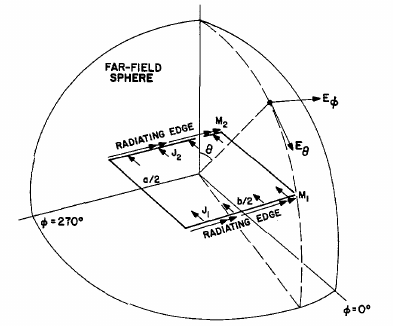
\includegraphics{microstrip_rad.png}
          \centering
          \caption{Geometry Far-field pattern of a rectangular microstrip \cite{CaM:81}}
        \end{figure}
        \indent This section will show the far-field radiation pattern of a rectangular microstrip patch on $TM_{10}$ mode at the radiating edge\cite{CaM:81}
        \begin{equation}
          E_{\theta} = - \frac{jV_0k_0ae^{-jk_0r}}{\pi r} \cos(kt\cos\theta) \frac{\sin[k_0 \frac{a}{2} \sin\theta\sin\phi]}{k_0 \frac{a}{2} \sin\theta\sin\phi}\cos(k_0\frac{b}{2}\sin{\theta}\cos{\phi})\cos{\phi}, (0 \leq \theta \leq \frac{\pi}{2})
        \end{equation}
        \begin{equation}
          E_{\phi} = \frac{jV_0k_0ae^{-jk_0r}}{\pi r} \cos(kt\cos\theta) \frac{\sin[k_0 \frac{a}{2} \sin\theta\sin\phi]}{k_0 \frac{a}{2} \sin\theta\sin\phi}\cos(k_0\frac{b}{2}\sin{\theta}\cos{\phi})\cos{\theta}\sin{\phi}, (0 \leq \theta \leq \frac{\pi}{2})
        \end{equation}
      
  \newpage

    \subsection{Q Factor}
      \indent There are 4 main loss that should be considered\cite{NoK:05}
      \begin{itemize}
        \item $Q_{rad}$ is radiation loss due to a loss which propagates into a space
          \begin{equation}
            %\begin{aligned}
              Q_{rad} = \frac{3}{16}\frac{\epsilon_r}{p}\frac{a_e}{b_e}\frac{\lambda_0}{h}\frac{1}{1-\frac{1}{\epsilon_r\mu_r}+\frac{2}{5\epsilon_r^2\mu_{r}^2}}
            %\end{aligned}
          \end{equation}
          \indent where $a_e$,$b_e$,$h$ is the effective length, width and thickness of the antenna respectively,
          $p$ is the ratio of the power that radiated by the patch antenna to the power radiated by an equivalent dipole\cite{NoK:05}
        \item $Q_{sw}$ is surface-wave loss which represents the amount of power coupled into space waves
          \begin{equation}
            Q_{sw} = Q_{rad}(\frac{\eta_r^0}{1-\eta_r^0})
          \end{equation}
          \indent where $\eta_r^0$ is the radiation efficiency without dielectric or conductor loss
        \item $Q_d$ is dielectric loss which defined as the ratio (or angle in a complex plane) of the lossy reaction to the electric field E in the curl equation to the lossless reaction
          \begin{equation}
            Q_d = \frac{1}{\tan\delta}
          \end{equation}
        \item $Q_c$ is metalization loss
        \begin{equation}
          Q_c = h\sqrt{\mu\pi{f}\sigma}
        \end{equation}
      \end{itemize}
      \indent The total quality factor of the antenna can be given by using this formula.
      \begin{equation}
        \frac{1}{Q} = \frac{1}{Q_{rad}} + \frac{1}{Q_{sw}} + \frac{1}{Q_d} + \frac{1}{Q_c}
      \end{equation}

  \newpage

  \subsection{Fringing Effect of the Microstrip Antenna}
    \indent Because of fringing effect, this will cause many phenomenas such as Effective length extension, 
            dielectric constant distortion and resonance frequency distortion\cite{CoB:05}
    
    \subsubsection{Effective Length Extension}
      \begin{figure}[ht]
        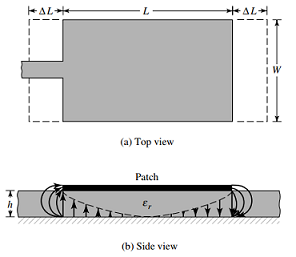
\includegraphics{fringingeffect.png}
        \centering
        \caption{The fringing effect that cause to length extension}
      \end{figure}
      \indent The length is extended because of fringing effect, that spreading at the edge of all sides so
              $L_{eff} = L + 2\Delta L$\cite{CoB:05} 
      \begin{equation}
        \frac{\Delta l}{h}=0.412\frac{(\epsilon_{r(eff)}+0.3)(\frac{W}{h} + 0.264)}{(\epsilon_{r(eff)}-0.258)(\frac{W}{h} + 0.8)}
      \end{equation}

    \subsubsection{Dielectric Constant Distortion}
      \begin{figure}[ht]
        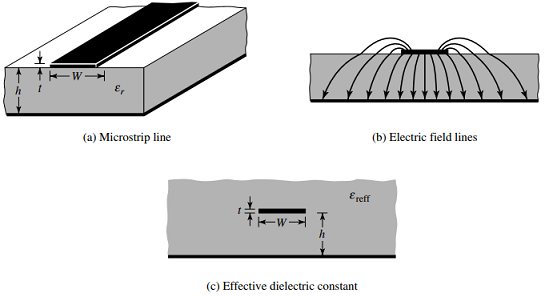
\includegraphics{dielectivef.png}
        \centering
        \caption{The fringing effect that cause to length extension}
      \end{figure}
      \indent Due to the electric field is not only happened inside the microstrip line, there's a leakage electric field in the air,
              so the dielectric that will be used for calculating will need to be reconsidered as follow\cite{CoB:05}
      \begin{equation}
        \epsilon_{reff} = \frac{\epsilon_{r} + 1}{2} + \frac{\epsilon_{r} - 1}{2}[1 + 12\frac{h}{W}]^{-0.5}
      \end{equation}

    \subsubsection{Resonance frequency distortion}
        \indent In $TM_{010}$ mode, the resonant frequency is given by
        \begin{equation}  
          f_{r(010)} =  \frac{1}{2 L\sqrt{\epsilon_{r}}\sqrt{\epsilon_{\mu_{0}\epsilon_{0}}}}= \frac{\upsilon_{0}}{2L\sqrt{\epsilon_{r}}}
        \end{equation}
        \indent With fringing effect, the equation will be given by
        \begin{equation} 
          f_{r(010)} =  \frac{1}{2 L_{eff}\sqrt{\epsilon_{r(eff))}}\sqrt{\epsilon_{\mu_{0}\epsilon_{0}}}}=\frac{1}{2(L + 2\Delta L)\sqrt{\epsilon_{r(eff)}}\sqrt{\epsilon_{\mu_{0}\epsilon_{0}}}}
        \end{equation} 
  
  \newpage

    \subsection{Phased Array Antena}
      In phased array antenna principle, there are 2 main factor in the equations. First one is an element factor which is the factor that come from only one antenna itself and the another factor is called array factor which is come from the effect of multiple antennas combining together.
      \begin{equation} 
        S(\vartheta)=S_{e}(\vartheta)S_a(\vartheta)  \label{ii}
      \end{equation}
        Whereas \\[1ex]
        \indent $S_{e}$ is a radiation pattern from only one element\\
        \indent $S_{a}$ is a element factor with
        \begin{equation} 
          S_{a}(\vartheta) = \sum\limits_{i=1}^K a_{i}e^{jk(K-i)dsin(\vartheta)}
        \end{equation}
        \indent $a_{i}$ is an amplitude taper.\\
        \indent $K$ is a number of array antenna.\\
        \indent $d$ is a distance of each antenna.\\
        \indent $\vartheta$ is a wavefront angle

  \newpage

  \section{Preliminary results}
    \indent This project results will consist of
    1) a simulation program that have ability  to simulate a microstrip from the given parameters.
    2) an phased antenna that could steer its direction to the desired point 
    
    \subsection{Simulation Application}
      \indent By using all the parameters that required to design the antenna, this simulation application will provide
              all the data from the algorithm that was proposed from the past. There are many techniques to simulate the antenna
              as Finite Element(FE), Method of Moments(MoM), or Numerical Method. However, the technique that will be used is one
              of those. In order to inspect on its correctness, the standard simulation application will be required to 
              compare. Consequently, the antenna results is expected to have similar outcomes as well.
    
    \subsection{Microstrip Antenna}
      \indent It's expected that a patch antenna should be have an impedance of zero Ohm at 5.6 GHz frequency
      \begin{figure}[ht]
        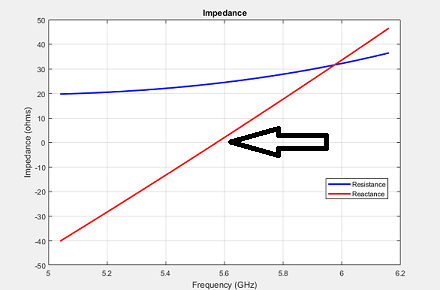
\includegraphics{Impedance.png}
        \centering
        \caption{The designed antenna's impedance should have approximately 0 Ohm reactance at 5.6 GHz}
        %\label{fig:1}
      \end{figure}

      \begin{figure}[ht]
        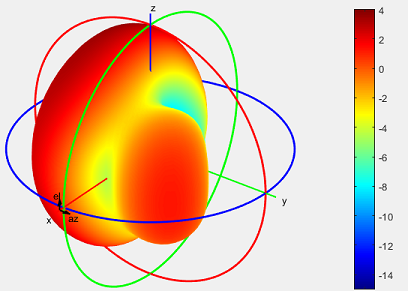
\includegraphics{Radiation_pattern}
        \centering
        \caption{The designed antenna's radiation pattern like the analysis}
        %\label{fig:2}
      \end{figure}

  \newpage

    \subsection{Array Antenna Patern}
      \begin{figure}[ht]
        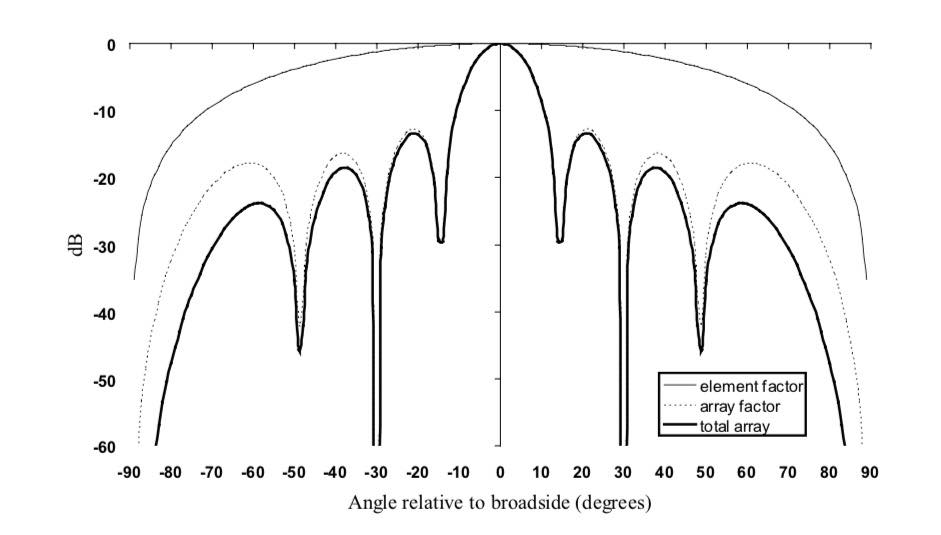
\includegraphics[scale=0.5]{no_taper}
        \centering
        \caption{Power radiation pattern without amplitude taper aka. $\forall a_{i} = 1$}
        %\label{fig:3}
      \end{figure}

      \begin{figure}[ht]
        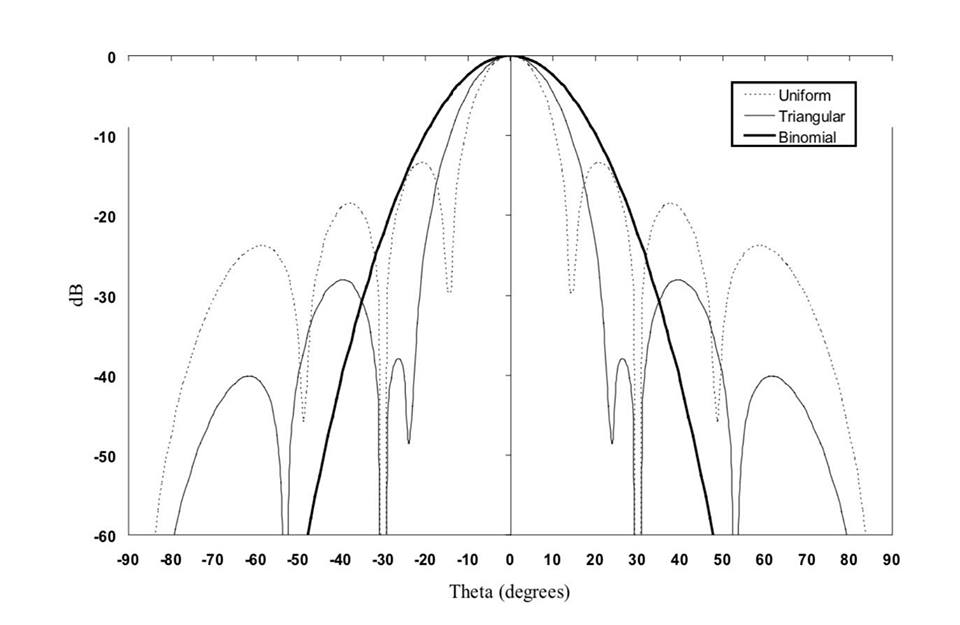
\includegraphics[ scale=0.5]{with_taper}
        \centering
        \caption{Power radiation pattern with amplitude taper of each type}
        %\label{fig:4}
      \end{figure}

  \newpage

  \section{Project overview}
    \subsection{Scope of work}
      \begin{itemize}
        \item An analysis of a microstrip antenna and phased array antenna
        \item A basic simulation application for finding antennas' radiation pattern
        \item A physical planar phased array microstrip patch antenna device with its test result.
      \end{itemize}

    \subsection{Expected outcomes}
      \indent It's expected that, the simulation application and the application that come from other author
      will have similar results. Also, the physical device should have a preliminary result like those simulation
      applications as well.
  
  \newpage
    \begin{landscape}  
    \subsection{Project Plan}
      \begin{figure}[ht]
        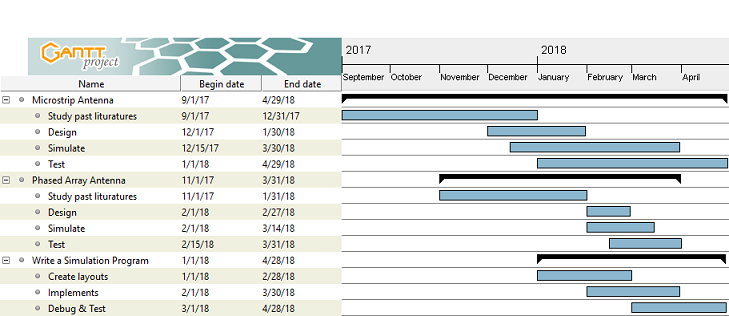
\includegraphics{gantt.png}
        \centering
        \caption{The project plan for the phased array antenna project}
        %\label{fig:1}
      \end{figure}
    \end{landscape}
  
  \newpage

  \bibliography{ref} 
  \bibliographystyle{ieeetran}

\end{document}
